\onecolumn

\section{Examples of more complex queries}
\label{example_scripts}
%|-----------------------------|
%| Python GSMF example script. |
%|-----------------------------|
\noindent {\bf Python - Galaxy stellar mass function}. This
example\footnote{Which can also be downloaded
here: \url{http://icc.dur.ac.uk/Eagle/Database/GSMF.py}} replicates Fig. 4
from \cite{Schaye2015} comparing the galaxy stellar mass function at $z=0.1$
({\tt SnapNum}$~=27$) in 30~pkpc apertures for three of the \eagle
simulations. The link to the database is created with the module {\sc
eagleSqlTools} available from the release website\footnote{Or directly here:
\url{http://icc.dur.ac.uk/Eagle/Database/eagleSqlTools.py}} (this module serves as an
interface to access the \eagle database). After the connection is established
(on line 9), the module can submit queries to the database. Each of the chosen
table properties (in this case we have only chosen the galaxy stellar masses)
are returned in a dictionary that can be then manipulated like any other {\sc
python} dictionary. We use the {\tt GROUP BY} \sql keyword to bin the data directly on the
server and reduce the amount of data being downloaded. The output created by this script is shown in
Fig.~\ref{fig:gsmf}.
\scriptsize
\pythonexternal{example_scripts/GSMF.py}
\normalsize
\setcounter{figure}{0}
\begin{figure}[t]
\centering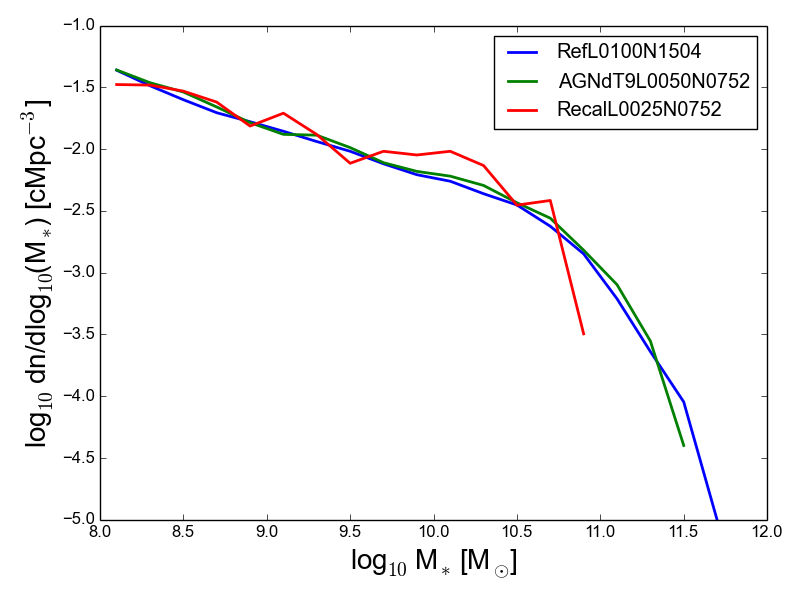
\includegraphics[width=8cm,angle=0]{example_scripts/GSMF}\vspace{-0.1cm}
\caption{Figure created by the {\sc python} script.}
\label{fig:gsmf}
\end{figure}
\normalsize
\FloatBarrier
\pagebreak

%|-----------------------------------------------------|
%| SQL black hole mass vs stellar mass example script. |
%|-----------------------------------------------------|
\noindent {\bf SQL - Black hole mass vs. stellar mass}. This example
replicates Fig. 10 from \citet{Schaye2015} showing the black hole mass as a
function of stellar mass at redshift $z=0.1$ ({\tt SnapNum}$~=27$) for 
the reference (L0100N1504) run. As mentioned in Section \ref{caveats}
we use the black hole subgrid mass, {\tt BlackHoleMass}, and treat the stellar mass of a galaxy
as the mass contained within a 30~pkpc aperture. {\bf SubHalo} table properties are connected to the {\bf
Aperture} table via each galaxy's unique \GalaxyID. 

\sqlstyle
\footnotesize
\begin{lstlisting}[numbers = none]
-- Select the quantities we want
SELECT      
	AP_Star.Mass_Star as sm,      
	SH.BlackHoleMass as bhm
-- Define aliases for the two tables      
FROM      
	RefL0100N1504_Subhalo as SH,      
	RefL0100N1504_Aperture as AP_Star
-- Apply the conditions        
WHERE      
	SH.SnapNum = 27                     -- z=0.1
	and SH.GalaxyID = AP_Star.GalaxyID  -- Match galaxies to Aperture table
	and AP_Star.ApertureSize = 30       -- Select aperture size to be 30 pkpc
	and AP_Star.Mass_Star > 0           -- Only return stellar masses > 0
	and SH.BlackHoleMass > 0            -- Only return black hole masses > 0
\end{lstlisting}

%|-------------------------------------------------|
%| SQL galaxy size vs stellar mass example script. |
%|-------------------------------------------------|
\normalsize
\noindent {\bf SQL - Galaxy size vs. stellar mass}. This example
         is similar to Fig. 9 from \citet{Schaye2015} comparing galaxy
         size as a function of stellar mass at redshift $z=0.1$ ({\tt
         SnapNum} $=27$) for each galaxy in the reference (L0100N1504)
         run. For galaxy sizes, we use the half mass radius of the
         galaxies from the {\bf Sizes} table. We
         connect them to the galaxy's stellar mass via the
         unique \GalaxyID identifier. As with the previous example, we
         must connect to the {\bf SubHalo} table to
         retrieve the {\tt SnapNum} value.

\sqlstyle
\footnotesize
\begin{lstlisting}[numbers = none]
-- Select the quantities we want
SELECT 
	AP.Mass_Star as sm, 
	SIZES.R_halfmass100 as size 
-- Define aliases for the three tables
FROM 
	RefL0100N1504_Subhalo as SH, 
	RefL0100N1504_Aperture as AP, 
	RefL0100N1504_Sizes as SIZES 
-- Apply the conditions
WHERE 
	SH.SnapNum = 27                  -- z=0.1
	and SH.GalaxyID = AP.GalaxyID    -- Match galaxies to Aperture table
	and SH.GalaxyID = SIZES.GalaxyID -- Match galaxies to Sizes table
	and AP.ApertureSize = 30         -- Select aperture size to be 30 pkpc
	and AP.Mass_Star > 0             -- Only return stellar masses > 0
\end{lstlisting}
\pagebreak

%|-----------------------------------|
%| SQL center offset example script. |
%|-----------------------------------|
\normalsize
\noindent {\bf SQL - Joining FOF and SubHalo tables}. 
This example shows how to join the properties of galaxies to their
parent FoF halo. In this case, we compute the offset between the
centre of the potential of the galaxy and the FoF halo. When dealing 
with positions within these volumes, remember to account for box
periodicity. In principle, it is not necessary to match the {\tt
SnapNum} of the tables as well as the {\tt GroupID}, but this
speeds up the query.

\sqlstyle

\footnotesize
\begin{lstlisting}[numbers = none]
-- Select the quantities we want
SELECT              
	SH.CentreOfPotential_x as sh_x,         
	SH.CentreOfPotential_y as sh_y,         
	SH.CentreOfPotential_z as sh_z,         
	FOF.GroupCentreOfPotential_x as fof_x,         
	FOF.GroupCentreOfPotential_y as fof_y,         
	FOF.GroupCentreOfPotential_z as fof_z,
	SH.MassType_Star as mstar, 
	FOF.GroupMass as fof_mass,
	square(SH.CentreOfPotential_x-FOF.GroupCentreOfPotential_x) 
		+ square(SH.CentreOfPotential_y-FOF.GroupCentreOfPotential_y)
		+ square(SH.CentreOfPotential_z-FOF.GroupCentreOfPotential_z) as dist
-- Define aliases for the two tables
FROM  
	RefL0050N0752_Subhalo as SH,              
	RefL0050N0752_FOF as FOF
-- Apply the conditions         
WHERE  
	SH.MassType_Star > 1.0e11    -- Only return stellar masses > 1.0e11
	and SH.SnapNum = 27          -- z=0.1
	and FOF.SnapNum = SH.SnapNum -- Join SnapNum to speed up query  
	and FOF.GroupID = SH.GroupID -- Join GroupID to speed up query
\end{lstlisting}

%|------------------------------------------------------|
%| SQL linking progenitor to decendants example script. |
%|------------------------------------------------------|
\normalsize
\noindent {\bf SQL - Linking a progenitor to its descendants}. 
This example shows how to select a random subset of Milky Way like
galaxies, and extract information about the location and specific star
formation rates (within a 30 pkpc aperture) of all their progenitors
above a stellar mass of $10^9\Msol$.

\sqlstyle
\footnotesize
\begin{lstlisting}[numbers = none]
-- Select the quantities we want
SELECT
	DES.GalaxyID,
	PROG.Redshift,
	PROG.MassType_DM,
	PROG.MassType_Star, 
	AP.SFR / (AP.Mass_Star+0.0001) as ssfr, 
	PROG.CentreOfPotential_x,
    	PROG.CentreOfPotential_y,
	PROG.CentreOfPotential_z
-- Define aliases for the three tables                      
FROM 
	RefL0100N1504_Subhalo as PROG,      
	RefL0100N1504_Subhalo as DES,
	RefL0100N1504_Aperture as AP
-- Apply the conditions           
WHERE 
	DES.MassType_Star between 1.0e10 and 6e10     -- Select Milky Way like stellar mass
	and DES.MassType_DM between 5.0e11 and 2.0e12 -- Select Milky Way like halo mass
	and DES.RandomNumber < 0.1                    -- Take a random subset of these
	and DES.SnapNum = 28                          -- At redshift z=0            
	and PROG.GalaxyID between DES.GalaxyID and DES.LastProgID -- Then find galaxy progenitors
	and AP.ApertureSize = 30                      -- Select aperture size to be 30 pkpc            
	and AP.GalaxyID = DES.GalaxyID                -- Match galaxies to Aperture table
	and AP.Mass_Star > 1.0e9                      -- Only return galaxies with stellar mass > 1e9
-- Order the output
ORDER BY 
	DES.MassType_Star desc,
	PROG.Redshift asc,
	PROG.MassType_Star desc
\end{lstlisting}
\twocolumn


